\chapter{Введение}
\label{ch:1}

Согласно теории Гинзбурга-Ландау обычно сверхпроводник вблизи \( T_c \) 
описывается одним комплексным параметром поля. Физика этих систем определяется 
двумя фундаментальными масштабными длинами, глубиной проникновения магнитного 
поля \( \lambda \) и длиной когерентности \( \xi \), а также коэффициентом 
\( \kappa \), который определяет реакцию на внешнее поле, разделяя их на 
категории следующим образом; сверхпроводники первого рода, где 
\( \kappa < 1/\sqrt{2} \) и второго рода, где \( \kappa > 1/\sqrt{2} \) 
\cite{bib:3}.

Свехрпроводники первого рода исключают слабые магнитные поля, в то время как 
сильные поля порождают формирования макроскопически нормальных областей с 
магнитным потоком \cite{bib:4}. Реакция сверхпроводников второго рода 
совершенно иная; ниже некоторого критического значения \( H_{c1} \), поле 
выталкивается. Выше этого значения сверхпроводник образует кристаллическую 
решетку или жидкостный вихрь, который имеет циркулирующее сверхпроводящее 
ядро проводящие магнитный поток через систему (!). И, наконец, при значении 
больше второго критического, \( H_{c2} \) сверхпроводимость разрушается. Эти 
различные ответы, как правило, рассматривается как последствия взаимодействия 
вихрей в этих системах, расход энергии на границе между сверхпроводящем и 
нормальном состояниях и термодинамической устойчивости вихревых возбуждений(!). 
В сверхпроводника второго рода расход энергии на границе между нормальной и 
сверхпроводящем состоянием является отрицательным, а взаимодействие между 
вихрями является отталкивающим.\cite{bib:3}. Это приводит к образованию 
устойчивых вихревых решеток и жидкостей. В сверхпроводниках первого рода 
ситуация противоположная; вихрь взаимодействия притягивающий (что делает их 
неустойчивыми против распада в один большой вихрь), а граница энергии между 
нормальным и сверхпроводящим состояниях положительно. С термодинамической 
точки зрения принципиальное отличие сверхпроводников первого рода от второго 
следующее: (i) В сверхпроводниках второго рода напряженности внешнего 
магнитного поля, необходимая, чтобы сделать образование вихревых возбуждений 
энергетически выгодными, \( H_{c1} \), меньше, чем термодинамическое 
магнитного поля \( H_{ct} \) (поле, энергетическая плотность равна энергии 
конденсации сверхпроводника, т.е. области, в которой равномерное 
сверхпроводящее состояние становится термодинамически неустойчивым); (ii) В 
сверхпроводниках первого рода напряженность поля требуется создание 
возбуждение вихря больше, чем критическое термодинамическое магнитное поле, 
т.е. вихри не могут образовываться. Можно выделить также специальный 
"нульмерный" пограничный случай, когда \( \kappa \) имеет критическое значение 
точно на границе первого/второго рода, что в самом общей модели ГЛ 
соответствует \( \kappa = 1/\sqrt{2} \). В этом случае вихри не 
взаимодействуют\cite{bib:5} в теории Гинзбурга-Ландау.

Вышеуказанные обстоятельства приводят к тому, что, в сильном внешнем магнитном 
поле, сверхпроводники первого рода обычно имеют тенденцию к минимизации 
энергии на границе между нормальной и сверхпроводящей фазой, что приводит к 
образованию крупных включений нормальной фазы, которые часто имеют слоистую 
структуру\cite{bib:4}. 

В последнее время наблюдается повышенный интерес к сверхпроводникам с 
несколькими сверхпроводящими компонентами. Основные ситуации, когда возникают 
множественные сверхпроводящие компоненты (i) многополосные сверхпроводники
\cite{bib:6,bib:7,bib:8,bib:9,bib:10,bib:11}, (ii) смеси независимых 
консервативных конденсатов, таких как прогнозируемая сверхпроводимость в 
атомарном водороде и богатых водородом сплавов \cite{bib:12,bib:13,bib:14} и 
(iii) сверхпроводников с другим типом симметрии, отличной от 
поперечно-волновой симметрии. В этой работе мы ориентируемся на случаи (i) и 
(ii). Принципиальная разница между случаями (i) и (ii) является отсутствие 
межкомпонентной джозефсоновской связи в случае с (ii).

Поэтому эти конденсаты не могут априори быть быть независимо сохраняющимися.
Это, на уровне эффективных моделей должно проявляться в довольно общем наличии 
межкомпонентной джозефсоновской связи.

В двухщелевых сверхпроводниках (i) сверхпроводящие компоненты происходят из
электронного куперовского спаривания в различных зонах \cite{bib:6}. Поэтому 
эти конденсаты не могут априори быть быть независимо сохраняющимися. Это, на 
уровне эффективных моделей должно проявляться в довольно общем наличии 
межкомпонентной джозефсоновской связи (!!!).

В случае (ii) две сверхпроводящие компоненты были предсказаны, происходящие 
из электронного и протонного куперовского спаривания в атомарном водороде 
или богатых водородом сплавов. В прогнозируемом жидкометаллическом дейтерии и 
сплавов богатых дейтерием, была предсказано существование электронной 
проводимости на сверхвысоких давлениях с дейтронной конденсацией  
\cite{bib:12,bib:13,bib:14}. Поскольку электроны не могут быть преобразованы в 
протонов или дейтрон с независимо сохраняющимися конденсатами(!!), и, 
следовательно, в эффективной модели Джозефсона межкомпонентная связь запрещена 
на основаниях симметрии. Этот эффект в настоящее время является предметом 
возобновлённых экспериментальных исследований. Ожидается, что они возникают 
при высоких, но экспериментально доступных давлениях (\( \approx 400 \)~ГПа). 
Текущие статические эксперименты сжатия достигают давлений 
\( \approx 350 \)~ГПа с давлением порядка 1 ТПа будучи ожидаемым в камере с 
алмазными наковальнями связи с недавними опытами получения ультра жёстких 
алмазов. Обсуждались похожие заряженные двухкомпонентные модели в контексте 
физики нейтронных звёзд, где они представляют сосуществующие протонную и 
\( \Sigma^\text{--} \)-гиперионную куперовскую пару внутри нейтронной звезды.
\cite{bib:15}. 

Недавно обсуждалось, что в многокомпонентных системах, где магнитный отклик 
гораздо сложнее, чем в обычных системах, и что разделение на сверхпроводники 
первого/второго рода не является достаточным условием для классификации.

Это большое разнообразие систем вызывает необходимость истолковать и 
классифицировать возможные магнитные отклики многокомпонентных 
сверхпроводников. Недавно он обсуждался, что в многокомпонентных системах, 
где магнитный отклик гораздо сложнее, чем в обычных системах, и что разделение 
на сверхпроводники первого/второго рода не является достаточным для 
классификации. Скорее всего, в широком диапазоне параметров, как следствие 
существовании трех основных масштабных длины, есть отдельный сверхпроводящий 
режим, при котором вихри имеют дальнодействующее притяжение, близкодействующее 
отталкивающее взаимодействие и форму вихревых узлов, погруженные в областях 
двухкомпонентного эффекта Мейснера (!!). \cite{bib:1,bib:2}. Последние 
экспериментальные работы \cite{bib:16,bib:17} выдвинули предположение, что 
это состояние реализуется в двухщелевом материале \( MgB_2 \), что вызвало 
растущий интерес к этой теме. В частности были подняты вопросы по поводу того, 
что сверхпроводимости типа 1,5 (как это было названо Мощалковым в 
al\cite{bib:16}, последнюю работу смотрите\cite{bib:18}) возможна даже в 
случае различных неисчезающих связей (например, внутренняя джозефсоновская 
связь, связь смешанных градиентов и т.д.) сверхпроводящими компонентами в 
разных диапазонах.

В этой работе мы приводим исследование появления сверхпроводимости типа 1,5 с 
особым упором на случаи многополосной сверхпроводимости, демонстрируя 
сохранение этого типа сверхпроводимости в присутствии различных видов 
межкомпонентных соединений (например, межзонное джозефсоновской связи, 
смешанных градиентных связей, плотность-плотность, и другие виды соединения).

\section{Сверхпроводимость типа 1,5}
\label{sec:1-1}

В принципе краевая задача в уравнении типа Гинзбурга-Ландау в присутствии 
оборота фазы, без строгого взгляда, сводится к одномерной задачи в целом.

Возможность нового типа сверхпроводимости, отличного от первого и второго рода 
в многокомпонентных системах \cite{bib:1,bib:2} основана на следующих 
соображениях. В принципе краевая задача в уравнении типа Гинзбурга-Ландау в 
присутствии оборота фазы, без строгого взгляда, сводится к одномерной задачи 
в целом. Кроме того, как указано в \cite{bib:1,bib:2}, в общей 
двухкомпонентной модели есть три фундаментальные масштабные длины, которые 
указывают

\begin{figure}[h!]
  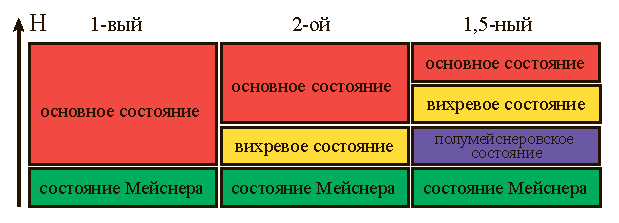
\includegraphics[width=.5\textwidth]{1-01}
  \caption{Сравнение фазовых диаграмм магнитных фаз чистых сверхпроводников
    первого, второго и полуторного рода при нулевой температуре. В 
    полумейсснеровском режиме макроскопическое разделение фаз в 
    двухкомпонентном Мейсснеровском состоянии и вихревых скоплений, где один 
    из режимов плотности подавляется внутренним перекрытием.}
  \label{fig:1}
\end{figure}

на невозможно параметризовать модель с точки зрения одного безразмерного 
параметра \( \kappa \). В случае, когда конденсаты не связаны межзонной 
джозефсоновской связью, при условии, что векторный потенциал этих масштабных 
длин является двумя независимыми величинами: длиной когерентности 
(устанавливается обратной массой соответствующей плотности скалярного поля) и 
глубиной проникновения магнитного поля (устанавливается обратной массой 
полученного калибровочного поля). В противоположность этому, в случае, когда к 
конденсаты соединяются с межзонными Джозефсоновскими условиями, можно не 
различить независимые длины когерентности и отнести их к различным 
конденсатам. Тем не менее, в этом случае колебания плотности также могут 
обладать двумя основными пространственными длинами \cite{bib:2}, в отличие от 
однокомпонентных теорий. Мы подробно остановиться на этом факте ниже. В 
\cite{bib:1,bib:2} вихревых решениях в двухкомпонентной теории были найдены 
компоненты, которые имеют немонотонное вихревое взаимодействие, с 
доминирующими частями отвечающие за дальнодействующее плотность-плотность 
взаимодействие и отталкивающей части  близкодействия типа ток-ток, и 
электромагнитного взаимодействия. Важным обстоятельством, которое было 
продемонстрировано, что эти вихри термодинамически стабильны, несмотря на 
существование притягивающего хвоста во взаимодействии.

Немонотонный межвихревой потенциал взаимодействия должен привести к 
образованию вихревых скоплений в слабомагнитном поле, погруженного в 
безвихревые пространство, эффект упомянутый в \cite{bib:1} как 
"полумейсснеровское состояние". На рисунке \ref{fig:1} схематические показана 
фазовая диаграмма сверхпроводника тип 1,5.

Если вихри образуют кластеры, то нельзя не использовать обычный одномерный 
аргумент относительно энергии сверхпроводника в нормальном состоянии границы 
раздела(!) для классификации магнитного отклика системы. Прежде всего, энергия 
на вихрь в таком случае зависит от того, является ли размещение вихря в 
кластере или нет: т.е. формирование единого изолированного вихря может быть 
энергетически невыгодным, в то время как формирование вихревых кластеров 
выгодно, потому что в кластере, где помещены вихри -- минимум потенциала 
взаимодействия, энергия на квант потока меньше, чем для изолированного вихря
(термодинамически немонотонный потенциал взаимодействия двух вихрей 
предусматривает, что наименьшей энергией на квант потока будет в случае 
равномерной сетке с шагом равным не менее двухчастичного межвихревого 
потенциала).

Таким образом, помимо энергии вихря в кластере, появляется дополнительная 
энергическая характеристика, связанная с границей кластера. Другими словами, в 
этой ситуации, для определения магнитного отклика системы недостаточно 
изучения краевой задачи и задачи одиночного вихря, в отличии от системы 
отдельных составляющих. Кроме того, в кластере система стремится к минимуму 
граничной энергии (так же, как и в сверхпроводниках 1-го рода), в то время 
нарушение структуры одного квантового вихря внутри кластера (аналогично 
сверхпроводимости второго рода с отрицательной энергией межфазного 
взаимодействия). Таким образом, увеличение магнитного поля образуется 
посредством фазового перехода первого рода. Магнитная фаза отлична от вихря в 
Мейснеровском состоянии, затем возникает макроскопическое фазовое 
распределение в двухкомпонентной области Мейснера и вихревых кластерах, где 
один из режимов плотностей подавляется основным перекрытием. Резюмируем 
основные свойства сверхпроводников первого, второго и полуторного рода в 
таблице I.

Существование термодинамически устойчивых сверхпроводящих типа 1,5 в конечном 
счете, зависит от существования немонотонного межвихревого потенциала 
взаимодействия. Важный вопрос как обобщается(!) данный эффект. В этой работе 
мы в основном сосредоточены на многополосных реализациях многокомпонентной 
сверхпроводимости и исследованию эффекта межзонной джозефсоновской связи, 
связи смешанного градиента, и связь типа плотность-плотность на вихревых 
взаимодействиях в двухщелевых сверхпроводниках. Покажем, что (i), когда эти 
соединения присутствуют, система по-прежнему может обладать три основными 
масштабными длинами, в отличие от двух пространственных в обычной 
однокомпонентной теории ГЛ; (ii) немонотонное взаимодействие возможно в 
широком диапазоне изменения параметров в этих моделях.

Структура данной работы состоит в следующем: В разделе II вводится модель. 
В разделе III мы представляем линейную теорию асимптотики вихревых полей в 
двухщелевых сверхпроводниках с различной межзонной связью.

Мы начинаем раздел III демонстрацией общего вида эффективного потенциала в 
двухщелевой (или в более общем -- двухзонном) свободной энергии 
Гинзбурга-Ландау, линейная теория дает при достаточно общих условиях две 
фундаментальные масштабные длины вариации плотности. 

Из линейной теории мы вычисляем потенциалы межвихревого дальнодействия 
используя двухкомпонентный метод обобщения точка-вихрь \cite{bib:19} и 
покажем, как потенциал немонотонного межвихревого взаимодействия является 
результатом взаимодействия двух фундаментальных масштабных длин: сверхтекучей 
вариации плотности и длины проникновения магнитного поля. Центральным пунктом 
этой части является как определяются масштабные длины в присутствии межзонной 
связи, а также возникновения "режима смешивания". Далее мы перейдём к 
количественному изучения влияния нескольких видов межкомпонентных связей, 
которые вполне единообразно возникают в двухкомпонентной теории.

В разделе III (d) показано, что смешанная градиентная связь может привести 
при определенных условиях к увеличения различия в вариации плотности 
характерных длин.

В разделе IV мы представляем большое численное исследование полной нелинейной 
задачи взаимодействия между парой вихрей.
